\documentclass[tikz,border=4pt]{standalone}
\begin{document}
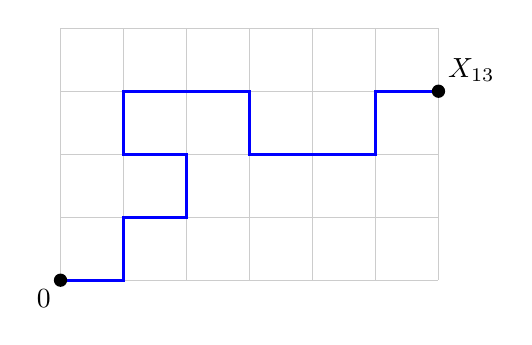
\begin{tikzpicture}[scale=0.8]
  \draw[step=1,gray!40] (0,0) grid (6,4);
  \draw[very thick,blue] (0,0)--(1,0)--(1,1)--(2,1)--(2,2)--(1,2)--(1,3)--(2,3)--(3,3)--(3,2)--(4,2)--(5,2)--(5,3)--(6,3);
  \fill (0,0) circle (3pt) node[below left] {$0$};
  \fill (6,3) circle (3pt) node[above right] {$X_{13}$};
\end{tikzpicture}
\end{document}
